\documentclass[a4paper,rep]{thesisby}

\usepackage[utf8]{inputenc}
\usepackage[english, russian]{babel}
\usepackage[hidelinks]{hyperref}
\hypersetup{
    allcolors=black
}

\usepackage{amsmath} % для математических формул и для автоматического добавления скобок при цитировании
\usepackage{IEEEtrantools} % для создания многострочных математических формул
\usepackage{commath} % для знака модуля
\usepackage{pdfpages} % для вставки pdf
\usepackage{epstopdf} % для вставки eps
\usepackage[justification=centering]{caption} % подписи таблиц посередине

\usepackage[figure,table]{totalcount} % для подсчёта числа картинок и таблиц
\usepackage{totcount}
\usepackage{totpages} % счётчик страниц. Желательно ставить последним пакетом в преамбуле

% для подсчёта числа источников литературы,
% но работает только после второй сборки
\newtotcounter{citenum}
\def\oldcite{}
\let\oldcite=\bibcite
\def\bibcite{\stepcounter{citenum}\oldcite}

% для склонений
%%http://www.linux.org.ru/forum/general/6993203#comment-6994589 (используется totcount)
\makeatletter
\def\formbytotal#1#2#3#4#5{%
    \newcount\@c
    \@c\totvalue{#1}\relax
    \newcount\@last
    \newcount\@pnul
    \@last\@c\relax
    \divide\@last 10
    \@pnul\@last\relax
    \divide\@pnul 10
    \multiply\@pnul-10
    \advance\@pnul\@last
    \multiply\@last-10
    \advance\@last\@c
    \total{#1}~#2%
    \ifnum\@pnul=1#5\else%
    \ifcase\@last#5\or#3\or#4\or#4\or#4\else#5\fi
    \fi
}
\makeatother

\graphicspath{{./figs/}}

\newcommand{\No}{\textnumero}

\begin{document}

\begin{titlepage}

\begin{center}
{
Министерство образования и науки Российской Федерации\\
Федеральное государственное автономное образовательное учреждение\\
высшего образования\\
<<Санкт-Петербургский политехнический университет Петра Великого>>
}
\end{center}
\vspace{0.5cm}

\hspace{-15mm}
\begin{tabular}{lcr} 
{
	\begin{tabular}[t]{l}
		УДК 004.051\\
		\No{1} \\
		Инв. \No{1} \\
	\end{tabular}
} & \hspace{40mm} & {
	\begin{tabular}[t]{l}
		У Т В Е Р Ж Д А Ю \\
		Зав. НИЛ <<Математическая биология\\
		и биоинформатика>>, ИПММ\\
		ФГАОУ ВО <<СПбПУ>>,\\
		д.б.н. \\
		\underline{\hspace{4cm}} М.~Г.~Самсонова\\
		<<\underline{\hspace{1cm}}>> \underline{\hspace{3cm}} 2016 г.
	\end{tabular}
}\\
\end{tabular}
\vspace{2cm}



\begin{center}
{
ОТЧЕТ\\
О НАУЧНО-ИССЛЕДОВАТЕЛЬСКОЙ РАБОТЕ\\
\vspace{3mm}
по теме:\\
<<Развитие метода разностной эволюции для поиска параметров математических моделей. Анализ эффективности различных методов>>\\
}
\end{center}

\vspace{3cm}


\hspace{15mm}
\begin{tabular}{ll}
{
	\hspace{60mm}
}&{
	\begin{tabular}[t]{l}
		Выполнил студент гр. \No{53601/4}\\
		{}\\
		\underline{\hspace{2cm}} А.~В.~Свичкарев\\
		<<\underline{\hspace{1cm}}>> \underline{\hspace{3cm}} 2016 г.
	\end{tabular}
}\\
{
	{}
}&{
}\\
{
	{}
}&{
	\begin{tabular}[t]{l}
		Руководитель НИР, к.б.н., в.н.с \qquad\\
		{}\\
		\underline{\hspace{2cm}} К.~Н.~Козлов\\
		<<\underline{\hspace{1cm}}>> \underline{\hspace{3cm}} 2016 г.
	\end{tabular}
}\\
\end{tabular}
\vspace{16mm}

\begin{center}
 Санкт--Петербург  2016
\end{center}

\end{titlepage}


\clearpage

\chapter*{РЕФЕРАТ}

% регистрируем счётчики в системе totcounter
\regtotcounter{totalcount@figure}
\regtotcounter{totalcount@table}       % Если поставить в преамбуле то ошибка в числе таблиц
\regtotcounter{TotPages}               % Если поставить в преамбуле то ошибка в числе страниц
\regtotcounter{citenum}

Отчёт \formbytotal{TotPages}{страниц}{а}{ы}{},
1 часть,
\formbytotal{totalcount@figure}{рисун}{ок}{ка}{ков},
\formbytotal{totalcount@table}{таблиц}{а}{ы}{}.
\formbytotal{citenum}{источник}{}{а}{ов}.
\bigskip

Ключевые слова:
МЕТОД ПОЛНОСТЬЮ ПАРАЛЛЕЛЬНОЙ РАЗНОСТНОЙ ЭВОЛЮЦИИ,
ИНТЕРПРЕТАТОР ЯЗЫКА R,
МЕЖПРОЦЕССНОЕ ВЗАИМОДЕЙСТВИЕ,
МАТЕМАТИЧЕСКОЕ МОДЕЛИРОВАНИЕ.

Целью работы является развитие метода ППРЭ,
а именно, разработка механизма
асинхронного взаимодействия метода
и минимизируемой функции.

Учитывая, что для решения задачи
минимизации произвольной целевой функции
не существует универсального алгоритма,
разработка и усовершенствование
методов минимизации остаётся актуальной задачей.

Разработанный механизм позволяет
сократить время вычислений
при использовании интерпретируемых языков,
например, системы статистических расчетов R
за счет единовременной загрузки
неизменяемых данных и
асинхронной загрузки переменных параметров.

Проведено тестирование быстродействия
новой реализации и показана эффективность улучшения.


\clearpage

\tableofcontents
\clearpage

\chapter*{ОБОЗНАЧЕНИЯ И СОКРАЩЕНИЯ}
\addcontentsline{toc}{section}{ОБОЗНАЧЕНИЯ И СОКРАЩЕНИЯ}

\textbf{РЭ} ---
разностная эволюция (Differential Evolution);

\textbf{DEEP, ППРЭ} ---
полностью параллельная разностная эволюция
(Differential Evolution Entirely Parallel);

\textbf{Интерпретатор} ---
программа, выполняющая пооператорную
(покомандную, построчную) обработку
и выполнение исходной программы или запроса;

\textbf{Асинхронная очередь задач} ---
паттерн в программировании,
представляющий структуру,
содержащую переиспользуемые
потоки параллельного исполнения
для вычислительных задач;

\textbf{Поток} ---
наименьшая единица обработки,
исполнение которой может быть назначено
ядром операционной системы;

\textbf{Пул потоков} ---
это коллекция потоков,
которые могут использоваться
для выполнения нескольких задач
в фоновом режиме.

\clearpage

\chapter*{ВВЕДЕНИЕ}
\addcontentsline{toc}{section}{ВВЕДЕНИЕ}

Проведение вычислительного эксперимента
с помощью математической модели
в большинстве случаев обходится значительно дешевле,
чем проведение соответствующего эксперимента
над реальным биологическим объектом,
кроме того некоторые условия
невозможно воспроизвести в лаборатории.
Параметры математической модели
должны быть выбраны таким образом,
чтобы получаемые решения
адекватно описывали объект в различных режимах.
Таким образом, разработка методов
и программ для решения обратной задачи
математического моделирования остается актуальной.

В большинстве случаев параметры модели
определяются минимизацией некоторой целевой функции,
описывающей отклонение решений от данных,
с учетом наложенных ограничений.

Методы оптимизации можно классифицировать
в соответствии с задачами оптимизации
на локальные методы,
которые сходятся к локальному экстремуму целевой функции
(в случае унимодальной функции,
экстремум единственный и одновременно
является глобальным экстремумом)
и глобальные методы,
которые стремятся к выявлению
глобальных тенденций поведения целевой функции
и поиску глобального экстремума.

Метод полностью параллельной разностной эволюции
(далее ППРЭ, DEEP) \cite{Kozlov11, Kozlov13}
является модификацией стохастического метода оптимизации,
предложенного в \cite{Storn95}.
DEEP представляет из себя эффективный метод
решения обратной задачи математического моделирования,
а именно модификация глобального стохастического метода.
Это значит, что он способен недетерминированно
(т.е. с использованием вероятностных методов)
находить экстремум для многоэкстремальных целевых функций
только с использованием вычисления целевой функции
в точках приближения без требования вычисления частных производных функции.

Программа DEEP успешно применялась для объяснения
резкого снижения экспрессии в gap генах
на ранних стадиях эмбриогенеза дрозофилы,
причиной которого стала нуль-мутация в гене \textit{Kr} \cite{kozlov2012modeling}.
Недавнее применение DEEP для нахождения
параметров в модели, основанной на
ДНК последовательностях с
регуляторной системой gap генов,
сделало возможным оценивать
вклад каждого сайта связывания
транскрипционного фактора \cite{kozlov2014sequence}.
Остальные применения DEEP
для различных задач описаны в
\cite{kozlov2013enhanced, ivanisenko2014new,
ivanisenko2013replication, kozlov2015differential}.

Целью работы является развитие метода ППРЭ,
а именно, разработка механизма асинхронного
взаимодействия метода и
минимизируемой функции отклонения
решения математической модели от
данных. За счет единовременной загрузки
неизменяемых данных и асинхронной
загрузки переменных параметров планируется
достигнуть сокращения времени вычисления
при использовании интерпретируемых
языков, например, для системы статистических
расчетов R.

Математические модели в биоинформатике
в большинстве случаев создаются
в таких компьютерных системах расчётов
как R, MATLAB, Octave и других.
Нахождение параметров в таких моделях
требует многократного вычисления решений,
что влечёт большие накладные расходы на запуск
того или иного интерпретатора.
Однако, интерпретатор может быть встроен в программу ППРЭ,
что позволит запускать нужное число копий один раз,
и, тем самым сократить время вычислений, для некоторых задач в разы.

Таким образом,
развитие методов решения обратной задачи математического моделирования
и эффективное распараллеливание существующих решений
является важным для исследований системной биологии.


\clearpage

\setcounter{figure}{0} \setcounter{table}{0} \setcounter{equation}{0}
\chapter*{ОСНОВНАЯ ЧАСТЬ}
\addcontentsline{toc}{section}{ОСНОВНАЯ ЧАСТЬ}

\section*{Теория метода DEEP}
\addcontentsline{toc}{subsection}{Теория метода DEEP}

Ниже приведено описание оригинального метода разностной эволюции
и его модификации DEEP.

Разностная эволюция (РЭ) ---
стохастический итерационный алгоритм минимизации,
предложенный Сторном и Прайсом в 1995 г.~\cite{Storn95}.

Метод оперирует случайно сгенерированными векторами параметров,
называемых индивидами. 
Под вектором понимается точка n-мерного пространства
из области определения целевой функции,
которую требуется минимизировать.
Множество индивидов называется популяцией.
Одна итерация популяции РЭ называется поколением.
Первое поколение генерируется случайным образом.
Новое поколение создаётся
по заданной схеме из индивидов текущего поколения.

Идея генерации нового поколения в оригинальном алгоритме
заключается в следующем.
Для каждого индивида текущего поколения
выбираются случайным образом 3 другие индивида
из поколения и вычисляется мутантный вектор по формуле:

\begin{equation} \label{mutant}
    v = v_1 + S \cdot (v_2 - v_3),
\end{equation}

где \begin{math}S\end{math} некоторая положительная константа масштабирования.

Производится операция скрещивания мутантного вектора с исходным,
замещением некоторых координат значениями из исходного вектора.
Полученный вектор называется пробным вектором.
Если значение целевой функции на нём стало меньше,
чем было на исходном, то пробный вектор добавляется в новое поколение.
Если нет, то в новое поколение переходит исходный индивид.
Таким образом, в каждом следующем поколение новые индивиды
стремится уменьшить значение целевой функции
и при определённых условиях может быть найден глобальный минимум.

Опишем две модификации РЭ, реализованные в \cite{KozlovThesis}.

\textbf{Скрещивание с учётом значения функционала:}

Используются два мутантных вектора,
на их основе определяется третий пробный вектор.
Первый мутантный вектор определяется
по соотношению \eqref{mutant},
второй мутантный вектор определяется
по аналогии с правилом треугольника \cite{zaharie2002parameter}:

\begin{IEEEeqnarray*}{rCl}
    z & = & \frac{v_1 + v_2 + v_3}{3}
    + (s_2 - s_1)(v_1 - v_2) \\
    && + (s_3 - s_2)(v_2 - v_3)
    + (s_1 - s_3)(v_3 - v_1), \nonumber
\end{IEEEeqnarray*}

где

\begin{equation*}
    s_i = \frac{\abs{F(q_i)}}
    {\abs{F(q_1)} + \abs{F(q_2)} + \abs{F(q_3)}},
\end{equation*}

для \begin{math}i = 1, 2, 3\end{math}.

Третий пробный вектор составляется из произвольного выбора
соответствующих координат мутантных векторов.
Пробный вектор переходит в новое поколение,
если значение функционала на нём меньше.

\textbf{Скрещивание для поддержания разнообразия индивидов:}

Адаптивная схема для изменения параметров
на основе управления разнообразием в популяции
была предложена в~\cite{fan2003trigonometric}.

Разнообразие популяции можно определить
через дисперсии параметров популяции:

\begin{equation} \label{varj}
    var_j = \frac{1}{NP} \sum_{i = 0}^{NP - 1}
    \left(q_{i, j} - \frac{1}{NP} \sum_{k = 0}^{NP - 1}q_{k, j}\right)^2
\end{equation}
где $j = 0, \dots, I - 1; I$ --- размер вектора параметров.

Введём отдельные константы масштабирования $S_j$ и
вероятности скрещивания $p_j$ для каждого параметра:

\begin{equation*}
    S_j = \left\{ \,
        \begin{IEEEeqnarraybox}[][c]{l?s}
            \IEEEstrut
            \sqrt{\frac{NP \cdot (c_j - 1) + p_j \cdot (2 - p_j)}
            {2 \cdot NP \cdot p_j}} &
            если $NP \cdot (c_j - 1) + p_j \cdot (2 - p_j) \geq 0$, \\
            S_{inf} & иначе.
            \IEEEstrut
        \end{IEEEeqnarraybox}
        \right.
\end{equation*}

\begin{equation*}
    p_j = \left\{ \,
        \begin{IEEEeqnarraybox}[][c]{l?s}
            \IEEEstrut
            -(NP \cdot S_j^2 - 1) +
            \sqrt{(NP \cdot S_j^2 - 1)^2 - NP \cdot (1 - c_j)} &
            если $c_j \geq 1$, \\
            p_{inf} & иначе.
            \IEEEstrut
        \end{IEEEeqnarraybox}
        \right.
\end{equation*}
где
\begin{equation*}
    c_j^{new} = \gamma \cdot \left(\frac{var_j}{var_j^{new}}\right)
\end{equation*}
где $\gamma$ --- новый управляющий параметр,
a $var_j$ определяется по \eqref{varj}.

Управляющие параметры инициализируются
случайным образом, после каждой итерации
обновляются константы масштабирования и
вероятности скрещивания по очереди.

\textbf{Полностью параллельная разностная эволюция:}

Метод РЭ имеет набор управляющих параметров,
которые влияют на скорость работы и сходимость.
К таким параметрам можно отнести
размер популяции, способ рекомбинации,
возраст старейших индивидов.

ППРЭ учитывает возраст индивида
в ходе эволюции.
Возраст индивида ---
число итераций, в течение которых
он не изменяется.
Большой возраст соответствует
попаданию в локальный минимум
функционала качества.
В ППРЭ место старейшего индивида
занимает индивид с наименьшим
значением функционала качества.

ППРЭ представляет собой модификацию метода РЭ,
поддерживающую распараллеливание
процесса вычислений.
Вычисления реализованы в несколько потоков
на многопроцессорных системах.
Каждый индивид помещается в очередь,
из которой извлекается и обрабатывается потоком.
Это позволяет существенно увеличить скорость работы.


\clearpage
\section*{Программная реализация DEEP}
\addcontentsline{toc}{subsection}{Программная реализация DEEP}

DEEP реализован на языке C с интерфейсом командной строки.
Пользователь задаёт команду с параметрами для тестирования,
которая запускает модель и выводит все измерения
разницы между решением модели
и экспериментальными данными для минимизации.
Исполнение начинается с блока инициализации,
в котором случайным образом генерируются
начальные вектора параметров индивида
длины $n$
с ограничениями сверху и снизу
на значения координат вектора.

Для ограничений в виде неравенств
применяются преобразования к равенству
с использованием тригонометрического синуса
или гиперболического тангенса\cite{Kozlov11}.

Текущее множество векторов параметров помещается
в блок популяции и на каждом из векторов
вычисляется целевой функционал.
Главный цикл алгоритма состоит из блоков
рекомбинации, оценивания и отбора.

Для параллельного вычисления индивидуальных решений
используется ThreadPool API из библиотеки GLib.
Задачи на вычисления целевого функционала,
указанного пользователем,
для каждого пробного вектора
помещаются в асинхронную очередь задач
и запускаются как только будет доступен свободный поток. 
Все потоки, которые начали своё выполнение
на текущей итерации должны завершиться
до следующей итерации.
Следующее поколение генерируется в блоке отбора
из популяции индивидов в соответствии
со значением целевого функционала.


\clearpage
\section*{Улучшение взаимодействия.\\Встраивание интерпретаторов}
\addcontentsline{toc}{subsection}
{Улучшение взаимодействия. Встраивание интерпретаторов}

Математические модели для DEEP,
функционал которых необходимо минимизировать
создаются в таких компьютерных системах расчётов
как R, MATLAB, Octave
и других интерпретируемых языках программирования.
Это реализуется в виде внешнего скрипта,
который указывается DEEP в качестве входного параметра.
Нахождение параметров требует
многократного вычисления решений,
что влечёт большие накладные расходы
на запуск и инициализацию интерпретатора.

Однако интерпретатор может быть встроен в DEEP.
Это позволит использовать процессорное время вычислений
более эффективно благодаря
улучшению взаимодействия между
методом оптимизации и
функционалом качества.
В работе был спроектирован и реализован
подход с использованием
асинхронной очереди задач и пула потоков
из библиотеки GLib.
Преимуществом использования GLib
является её кроссплатформенность
и принадлежность к свободному программному обеспечению.

В конфигурационном файле был добавлен
параметр числа потоков в пуле потоков,
который указывается пользователем
при старте DEEP.

\textbf{Опишем более подробно ход выполнения программы
при новом подходе.}

После начальной инициализации DEEP
и генерации начальной популяции,
создаётся пул потоков,
число потоков в котором равно
указанному пользователем числу в
конфигурационном файле.
В каждом потоке параллельно
запускается свой интерпретатор того языка,
на котором была реализована математическая модель.
В каждый интерпретатор загружаются
функции из скрипта
для вычисления значения функционала
на векторе параметров индивида.
Так как запускается интерпретатор
с интерфейсом командной строки,
необходимо создать потоки ввода-вывода,
для связи интерпретаторов
с главным потоком исполнения,
которому необходимо получить
результаты вычислений со всех интерпретаторов.
Векторы индивидов из поколения популяции
образуют задачу и
добавляются в асинхронную очередь задач.
Свободный поток из пула потоков
выбирает из очереди первую задачу
и вызывает в своём потоке
исполнение вычисления функционала
на данном векторе в интерпретаторе.

После вычисления интерпретатор
возвращает результат в
выходной поток к главному потоку выполнения,
задача считается выполненной.
Свободный поток выбирает следующую задачу
и таким образом всё повторяется,
пока в очереди не закончатся задачи.
DEEP создаёт новое поколение популяции
и весь процесс повторяется,
либо до указанного числа итераций или
пока не будет достигнута сходимость
значений функционала.

Как указывалось выше,
используются структуры и алгоритмы
\textbf{GLib}\cite{GLib}:

\begin{itemize}
    \item \textbf{Thread Pool} --- пул потоков;
    \item \textbf{Asynchronous Queue} --- асинхронная очередь задач;
    \item \textbf{IO Channel} --- поток ввода-вывода;
\end{itemize}


\clearpage
\section*{Тестовая функция}
\addcontentsline{toc}{subsection}{Тестовая функция}

В качестве тестовой функции для минимизации
использовалась смещённая функция Растригина $R$:

\begin{equation*}
    r = \sum_{i = 1}^{D}(x_i^2 - 10\cos(2 \pi x_i) + 10)
\end{equation*}

\begin{equation*}
    R = r\left(\frac{5.12 (x - o_r)}{100}\right) + 800
\end{equation*}

Вектор параметров $x$ был выбран размера 30.

Было проведено тестирование
аналогично описанному в разделе
Численные эксперименты.
Для каждого значения параметра
числа интерпретаторов было выполнено
по 10 запусков
с числом итераций и размером популяции
равным 100.
Однако не были получены
статистические различия.
Отсутствие эффекта
от оптимизации может
быть объяснено тем,
что служебные функции
выполняются значительно быстрее.

\begin{figure}[h]
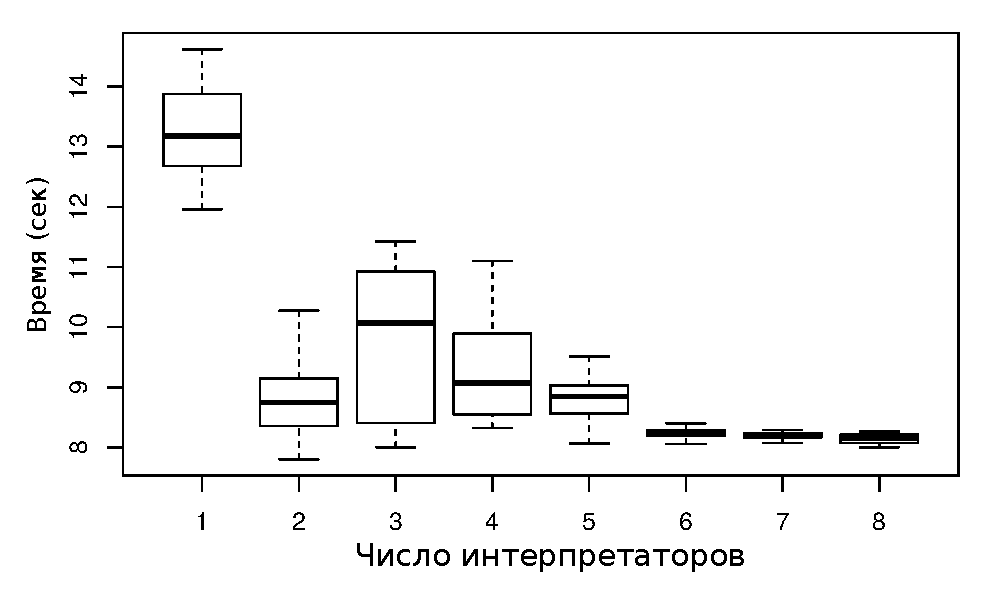
\includegraphics{rastrigin}
\caption{Медиана и полтора межквартильных расстояния
времени выполнения в зависимости от числа интерпретаторов}
\label{fig:rastriginboxplot}
\end{figure}

На рис.~\ref{fig:rastriginboxplot} видно,
что при увеличение числа интерпретаторов
время выполнения одинаковой задачи уменьшается.


\clearpage
\section*{Сегментация траекторий частиц}
\addcontentsline{toc}{subsection}{Сегментация траекторий частиц}

Обратной задачей математического моделирования
может являться выявление параметров взаимодействий биологических молекул,
которые не могут быть измерены напрямую из экспериментов.

Для тестирования программы использовалась
прикладная задача трэкинга частиц
и сегментации траекторий \cite{pisarev2015tracker}.

Исходными данными являются
серии снимков биологических макромолекул,
а именно эндосом эпидермального фактора роста
в клетках HeLa.

Первым этапом обработки происходит выделение
положения частиц из исходных снимков.
Затем с помощью стороннего программного обеспечения
производится построение траекторий.
Главной задачей является выяснить
как частицы движутся в клетке,
т.е. разбить траекторию на участки,
соответствующие либо диффузии,
либо направленному движению по микротрубочке.

Для последней задачи использовались
скрытые марковские модели,
что позволило получить
параметры движения и
построить вероятностную модель
биологического процесса.

Вероятности переходов и параметры движений
определяются из экспериментальных данных.
Скрипт для построения скрытой марковской модели
и использующий максимизацию правдоподобия
для определения параметров использует
метод ППРЭ и реализован на языке R.
Перед вычислением функционала качества
таблица траекторий подвергается предобработке.


\clearpage
\section*{Численные эксперименты}
\addcontentsline{toc}{subsection}{Численные эксперименты}

Тестирование проводилось на компьютере со следующими характеристиками:

\begin{table}[h]
\centering
\begin{tabular}{| c | c |}
    \hline
    Частота процессора & 3.7 ГГц \\ \hline
    Архитектура & 64-битная \\ \hline
    Модель процессора & Intel(R) Xeon(R) CPU E5-1620 v2 \\ \hline
    Число ядер & 8 \\ \hline
    Оперативная память & 64 Гб \\ \hline
    Объём жёсткого диска & 300 Гб \\
    \hline
\end{tabular}
\caption{Характеристики оборудования,
на котором проводилось тестирование}
\end{table}

Старой реализацией будем называть
изначальную реализацию,
где для вычисления функционала
на векторе параметров запускался
новый интерпретатор и
заново происходила загрузка
данных о траекториях.

Новым вариантом реализации
будем называть реализацию,
где используется очередь задач
и пул потоков,
интерпретаторы инициализируются
один раз и не подвергаются перезапуску,
то есть время жизни интерпретатора
завершается с окончанием оптимизации.

План тестирования заключался
в сравнение времени работы
старой и новой реализаций
при одинаковых параметрах.
Проводились многократные запуски
с целью подтверждения или опровержения
гипотезы о статистической значимости различий
времени работы реализаций.
Под нулевой гипотезой будет пониматься
различие математического ожидания
старой и новой реализаций.

Первым этапом численного эксперимента
было получение замеров времени
работы приложения
при различных комбинациях параметров.
Проводилось по 100 запусков
для каждого набора параметров.

Параметрами были выбраны следующие характеристики:

\begin{itemize}
    \item \textbf{Число потоков (\textit{i})}

        Для новой реализации этот параметр также
        обозначал размер пула потоков.
        Диапазон значений: 1-8.
    \item \textbf{Коэффициент размера популяции (\textit{M})}

        Размер популяции рационально выбирать
        пропорционально числу потоков,
        чтобы на каждый поток приходилась
        равная нагрузка при различном
        числе \textit{i}.

        Таким образом размер популяции равен:
        \begin{math}M * i\end{math}

        Тестирование проходило для значений:
        \begin{math}M = 5; M = 10\end{math}.
\end{itemize}

\break
На рис.~\ref{fig:m5}, рис.~\ref{fig:m10} представлены результаты тестирования:

\begin{figure}[!h]
\centering
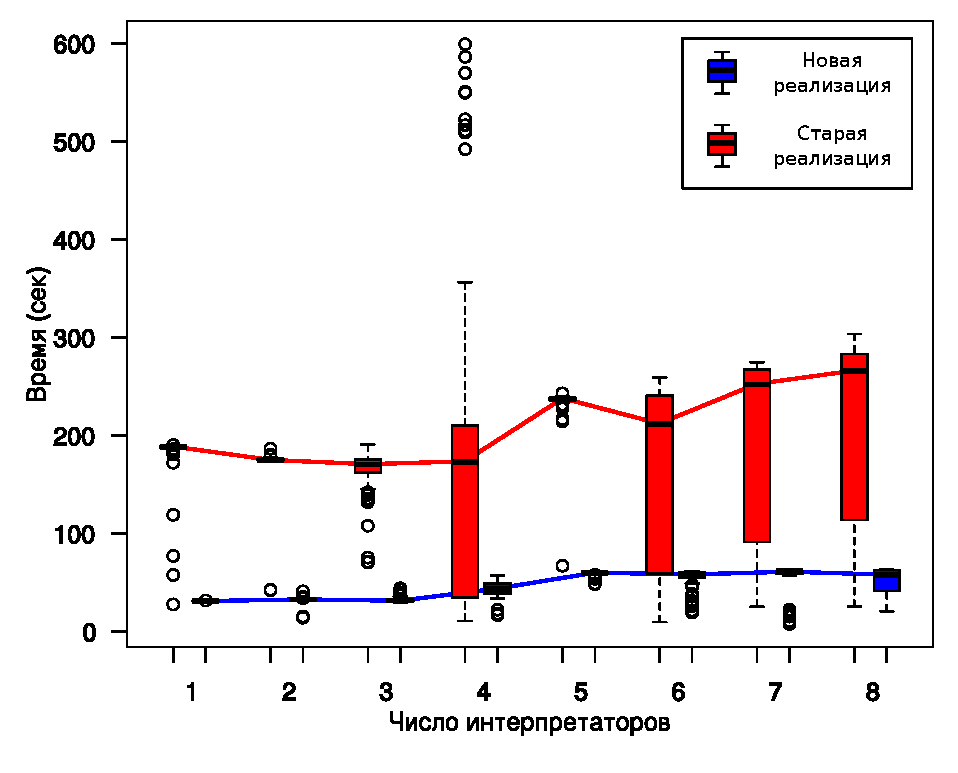
\includegraphics[width=0.74\textwidth]{m5}
\caption{Медиана и полтора межквартильных расстояния
времени выполнения при $M = 5$}
\label{fig:m5}
\end{figure}

\begin{figure}[!h]
\centering
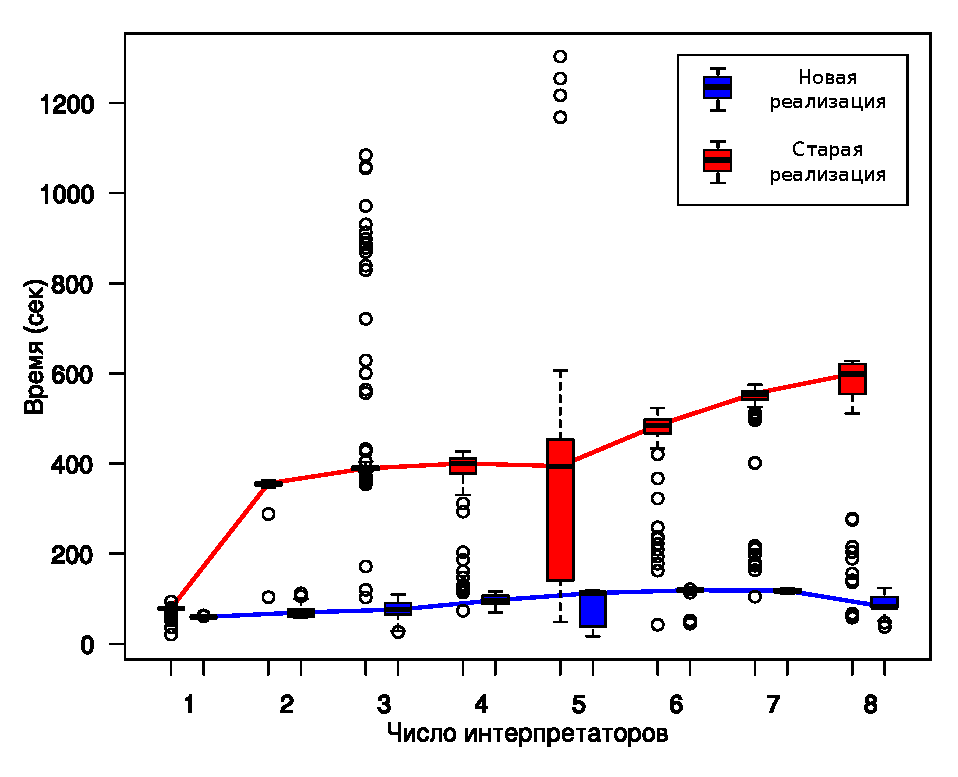
\includegraphics[width=0.74\textwidth]{m10}
\caption{Медиана и полтора межквартильных расстояния
времени выполнения при $M = 10$}
\label{fig:m10}
\end{figure}

Такую существенную разницу во времени выполнения
можно объяснить большими накладными расходами
на инициализацию на каждой итерации алгоритма
нового экземпляра интерпретатора
и освобождения ресурсов от старого,
больше не используемого экземпляра.
По большому разбросу значений
старой реализации можно предположить,
что существовали проблемы с конкуренцией
за ресурсы при инициализации интерпретаторов,
которые в некоторых случаях приводили к
существенному общему замедлению выполнения программы.
Из рисунков видно,
что в новой реализации разброс существенно меньше.

Разработанный механизм обеспечивает
четырёхкратный прирост производительности
на четырёх параллельных потоках
с четырьмя интерпретаторами по
сравнению со старой реализацией.

Было проверено, оказывает ли изучаемый параметр,
в данном случае это новый вариант реализации,
существенное влияние на интересующую нас
переменную, на время работы.
Проверка осуществлялась с помощью
критерия достоверно значимой
разности Тьюки
с уровнем значимости в 95\%.
Он необходим, чтобы посмотреть
где именно лежат статистические различия.

\begin{figure}[!h]
\centering
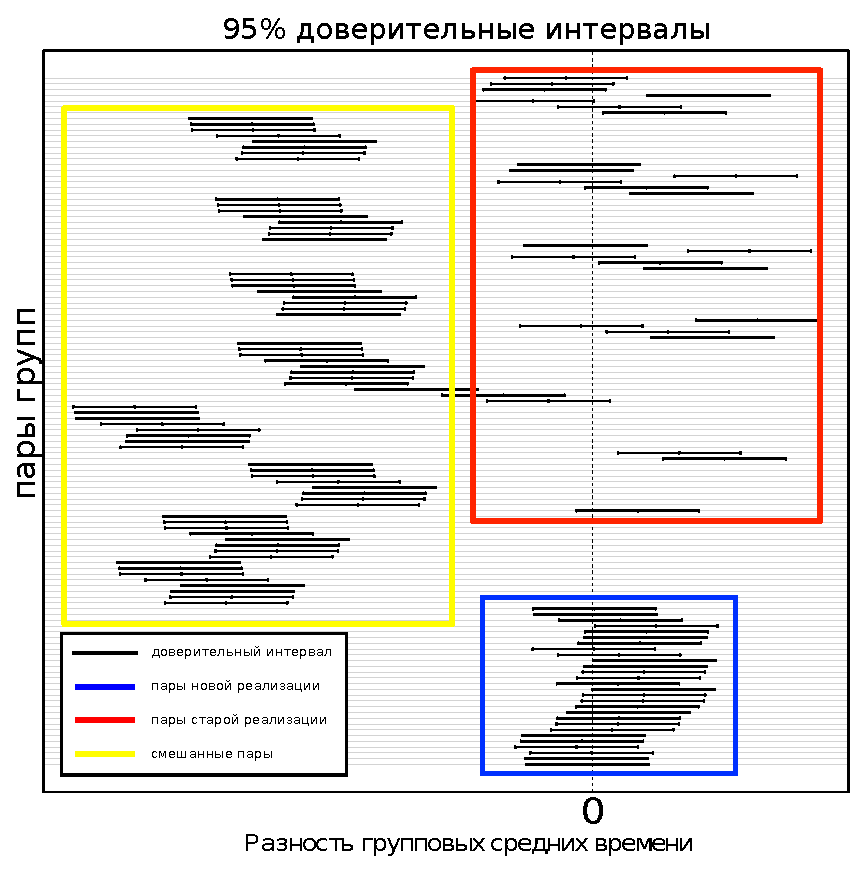
\includegraphics[width=\textwidth]{tukey}
\caption{График 95\% доверительных интервалов,
построенных по критерию Тьюки.
Цветными рамками обозначены группы сравниваемых пар.
Старая и новая реализации имеют статистически
значимую разницу}
\label{fig:tukey}
\end{figure}

Пунктирной вертикальной линией на рис.~\ref{fig:tukey}
показана нулевая разница между групповыми средними времени.
Если доверительный интервал включает 0,
это указывает на отсутствие различий
между соответствующими группами.

На рис.~\ref{fig:tukey} выделены три группы цветными рамками:
\begin{itemize}
    \item \textbf{Интервалы внутри красной рамки (справа вверху)} ---
        пары групп старой реализации с различным числом интерпретаторов.
        Интервалы лежат возле нуля, но присутствует
        некоторое разница, как в положительную сторону,
        так и в отрицательную. Это может объясняться
        конкуренцией интерпретаторов
        за вычислительные ресурсы и доступом к конфигурационным файлам
        при их одновременной инициализации.
    \item \textbf{Интервалы внутри синей рамки (справа внизу)} ---
        пары групп новой реализации с различным числом интерпретаторов.
        В данной группе различия минимальны,
        что является свидетельством оптимизации.
        В новой реализации инициализация интерпретаторов
        происходит единожды, поэтому
        узкое место не сильно замедляет работу
        при конкуренции, в дальнейшем
        интерпретаторы не так конкурируют за ресурсы.
    \item \textbf{Интервалы внутри жёлтой рамки (слева)} ---
        смешанные группы новой и старой реализации.
        Разница статистически значима,
        это означает, что оптимизация играет существенную роль.
\end{itemize}


\clearpage

\chapter*{ВЫВОДЫ}
\addcontentsline{toc}{section}{ВЫВОДЫ}

Исходя из полученных результатов
можно сделать следующие выводы:
\bigskip

\begin{enumerate}
    \item Использование интерпретируемого языка
    для описания математической модели
    не является препятствием для применения
    эффективного метода оптимизации
    и распараллеливания вычислений.
    Разработанный механизм обеспечивает
    четырёхкратный прирост производительности
    на четырёх параллельных потоках
    с четырьмя интерпретаторами
    по сравнению со старой реализацией.

    \item Реализованная интеграция
    сохраняет кроссплатформенность DEEP,
    так как в основе решения
    использовалась библиотека GLib,
    портированная на основные операционные системы.

\end{enumerate}


\clearpage

\chapter*{ЗАКЛЮЧЕНИЕ}
\addcontentsline{toc}{section}{ЗАКЛЮЧЕНИЕ}

Целью работы являлось развитие метода ППРЭ,
а именно, разработка механизма асинхронного взаимодействия
метода и минимизируемой функции отклонения
решения математической модели от данных.
За счет единовременной загрузки неизменяемых данных
и асинхронной загрузки переменных параметров
было достигнуто сокращения времени вычисления
при использовании интерпретируемых языков,
таких, как системы статистических расчетов R.

Метод полностью параллельной разностной эволюции
является модификацией стохастического метода оптимизации.
DEEP представляет из себя
эффективный метод решения обратной задачи
математического моделирования,
а именно модификация глобального стохастического метода.

Показана эффективность
оптимизации в сравнении с
прошлой реализацией.
Модификация ППРЭ
была разработана на основе
открытой кроссплатформенной
библиотеки GLib,
что сохраняет кроссплатформенность DEEP.

Использование интерпретируемого языка
для описания математической модели
не является препятствием для применения
эффективного метода оптимизации
и распараллеливания вычислений.
Разработанный механизм обеспечивает
четырёхкратный прирост производительности
на четырёх параллельных потоках
с четырьмя интерпретаторами
по сравнению со старой реализацией.

Работа развивает метод deep
в направлении улучшения интеграции,
что ведёт к увеличению количества
проверяемых гипотез.


\clearpage

\bibliographystyle{utf8gost71u}
\bibliography{citations}

\end{document}

